\chapter{Sample applications with color probabilities }\label{Appendix:4}

We present two potential applications of using the dwarf-giant difference in colors \jwone and \jwtwo, reduced proper motions in J-band (\ref{sec:RPM}) and combining color probabilities with a galactic model (\ref{sec:galactic_model}) .

\section{Reduced proper motions} \label{sec:RPM}

All of the Michigan stars are HD stars with GAIA parallaxes and proper motions. We cross-correlate the Michigan catalog with the GAIA First Data Release \citep[]{gaia1,gaia2,Lindegren2016}.  In Figure 8, we plot the standard reduced proper motion (${rpm}_J$) for the Michigan stars as a function of \jwtwo for spectral types from G0--K5 and luminosity class, using GAIA proper motions. In Figures \ref{fig:absolute_j_jw1} and D.2, we plot the absolute J-band magnitudes for the Michigan stars as function of \jwtwo for spectral types from G0--K5 and luminosity class, using GAIA parallaxes. From these plots, we see that the classification success rate of the Michigan catalog is high, but not perfect.

\section{Galactic population model} \label{sec:galactic_model}

We are considering also further finessing the color-luminosity class probability by relating color with position in the sky using a a synthetic galactic model of the Milky Way called TRILEGAL, but leave this for future work. Incorporating giant/dwarf population statistics, such as luminosity class number density as a function sky area, should help to further improve color as a tool to predict luminosity class, and for application to future surveys.

We plan to pick an ecliptic pole field as an application of calculating probabilistic luminosity class membership in a Bayesian framework. In particular, our priors are the mean and robust standard deviation of colors of each luminosity class as calculated in Chapter (\ref{subsec:median_stats}). We plan to use the TRILEGAL source counts to normalize these distributions with respect to one another, and integrate over a sample photometric measurement and its uncertainty.

% FIGURES =================

\begin{figure*}[t] 
  \begin{center}
      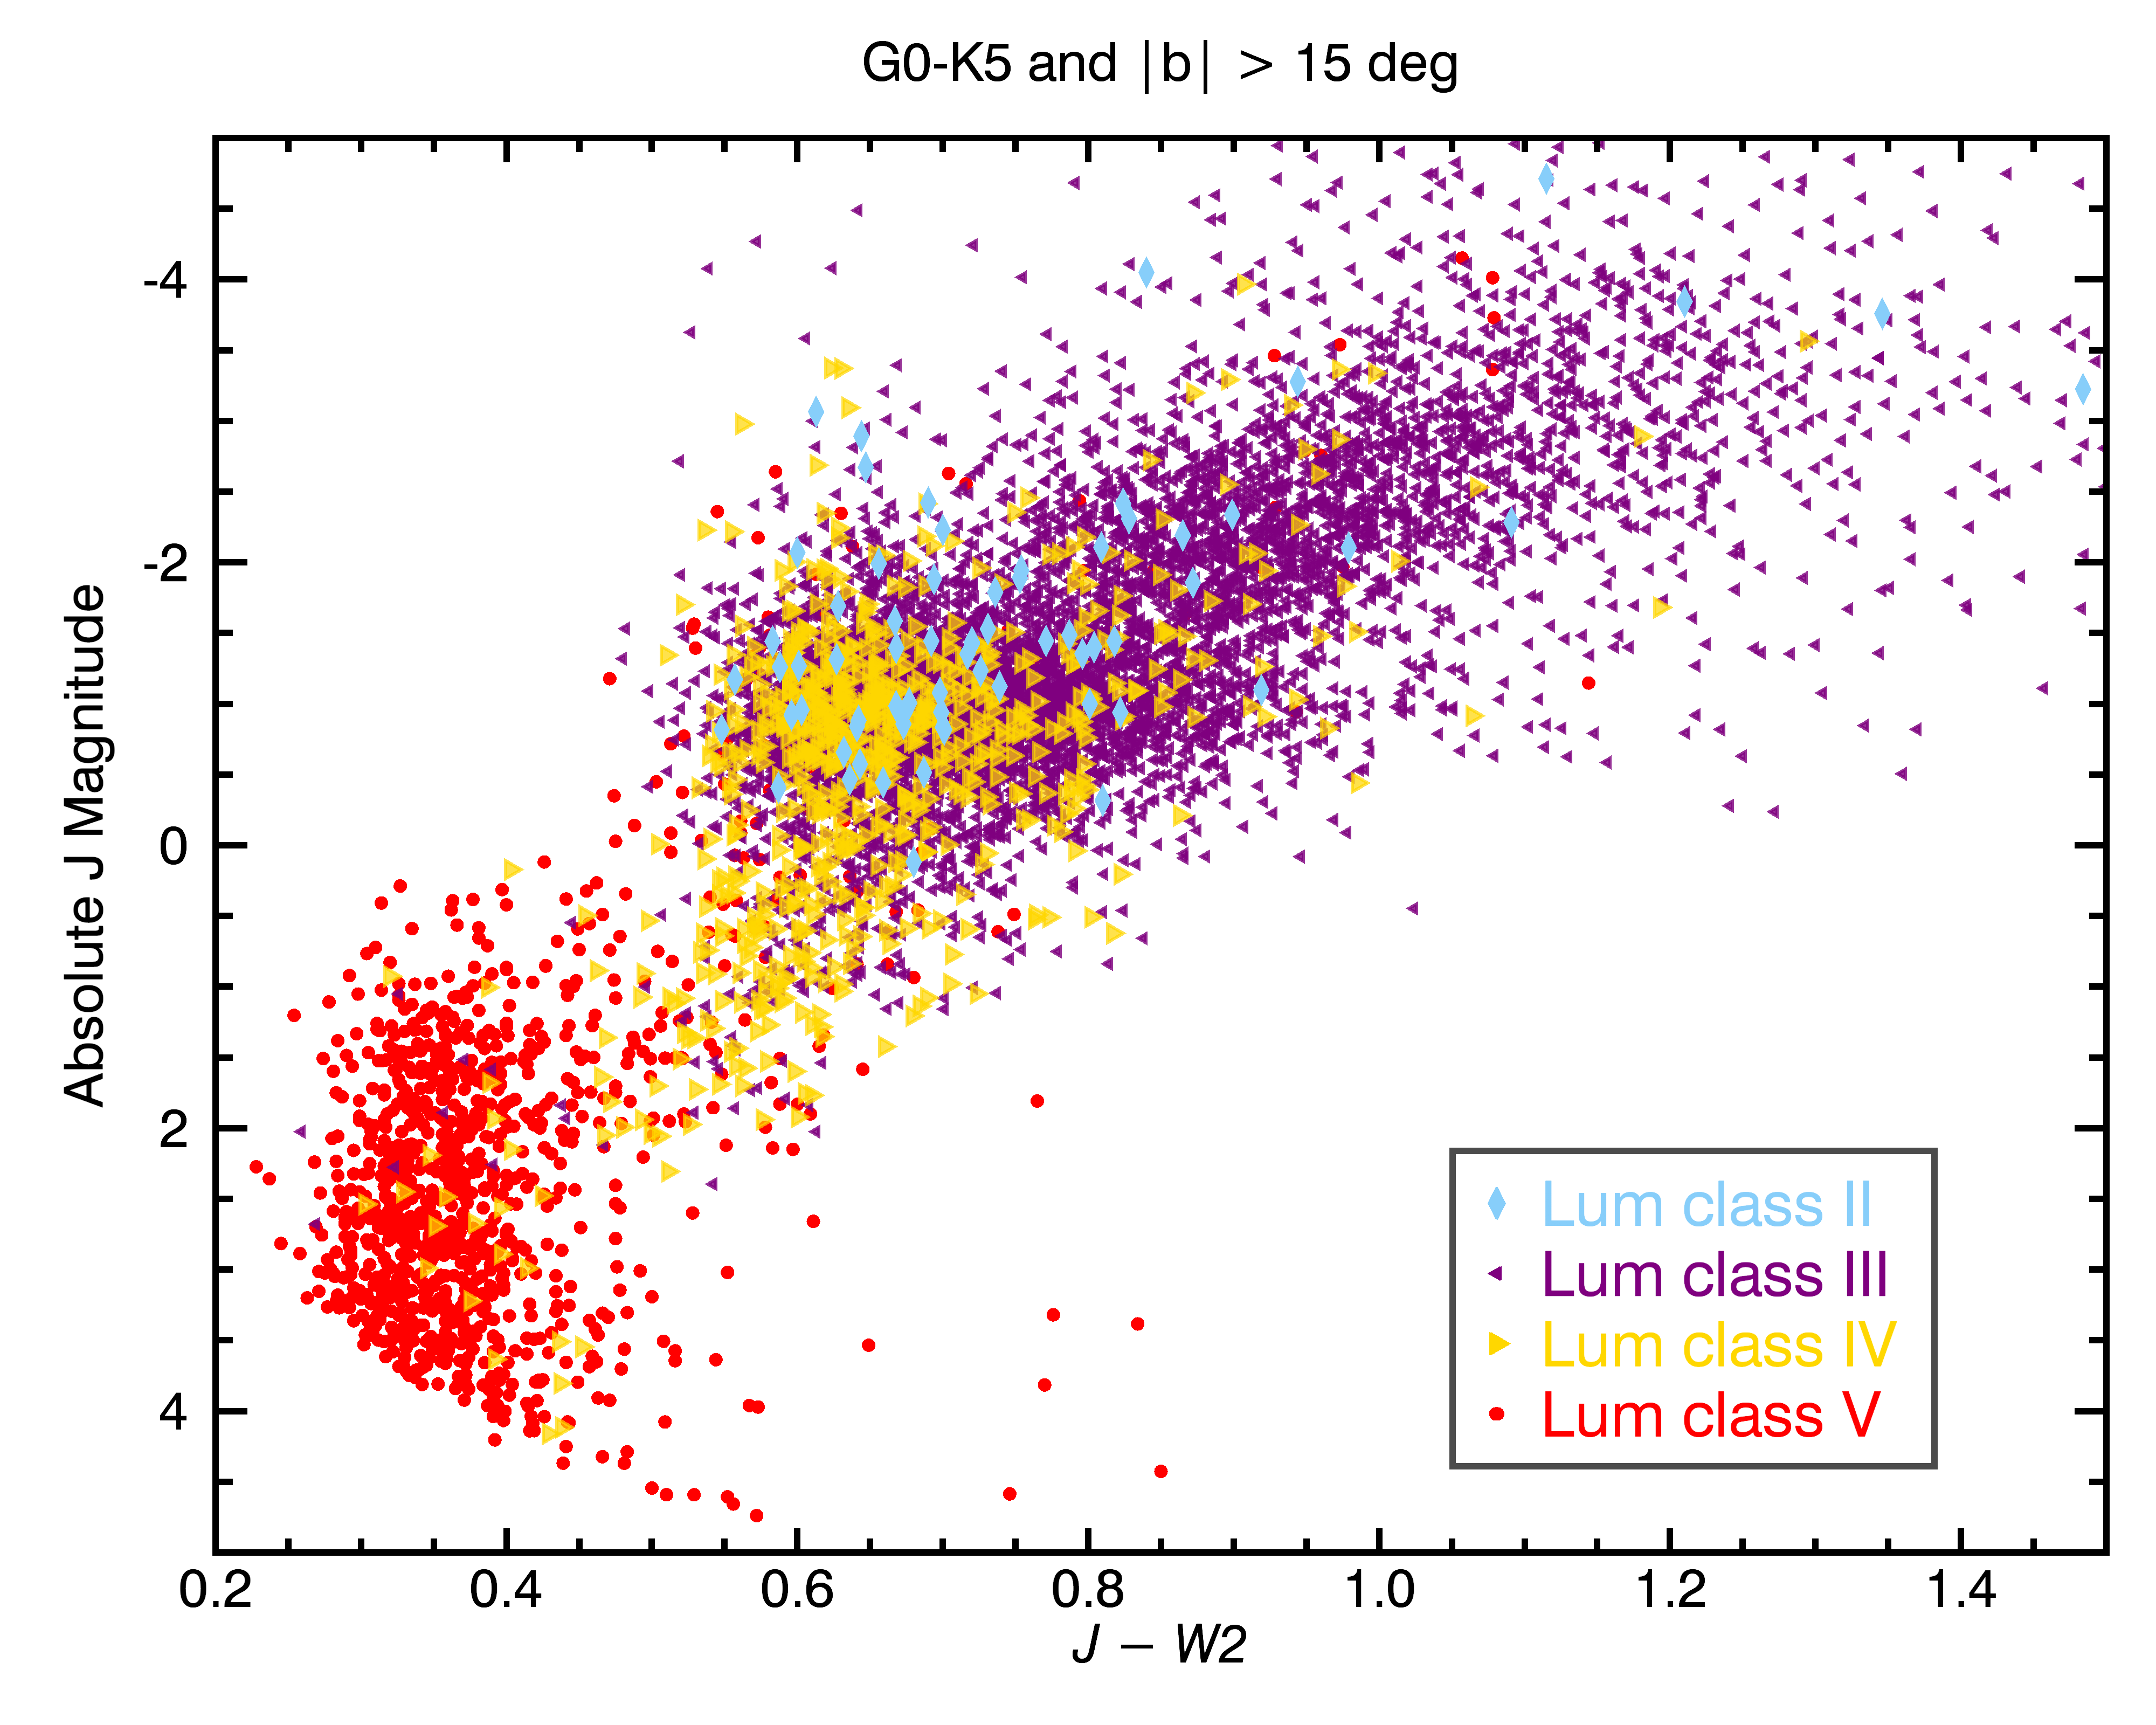
\includegraphics[width=1.0\textwidth,clip=true]{Figures/absolute_j/plot-J-W2-G0-K5-b15-abs-J.png}
 \end{center}
 \caption{Reduced $J$-band proper motion plot using \textit{GAIA} DR1 proper motions as a function of $J-W2$ color for Michigan Spectral Atlas stars with spectra types between G0 and K5 and galactic latitudes $|b|>15\deg$.  The different colors correspond to the different luminosity classes, and show a relatively clear separation between dwarfs and (sub-)giants.}\label{fig:absolute_j_jw1}
\end{figure*} 

\begin{figure*}[t] 
\begin{center}
    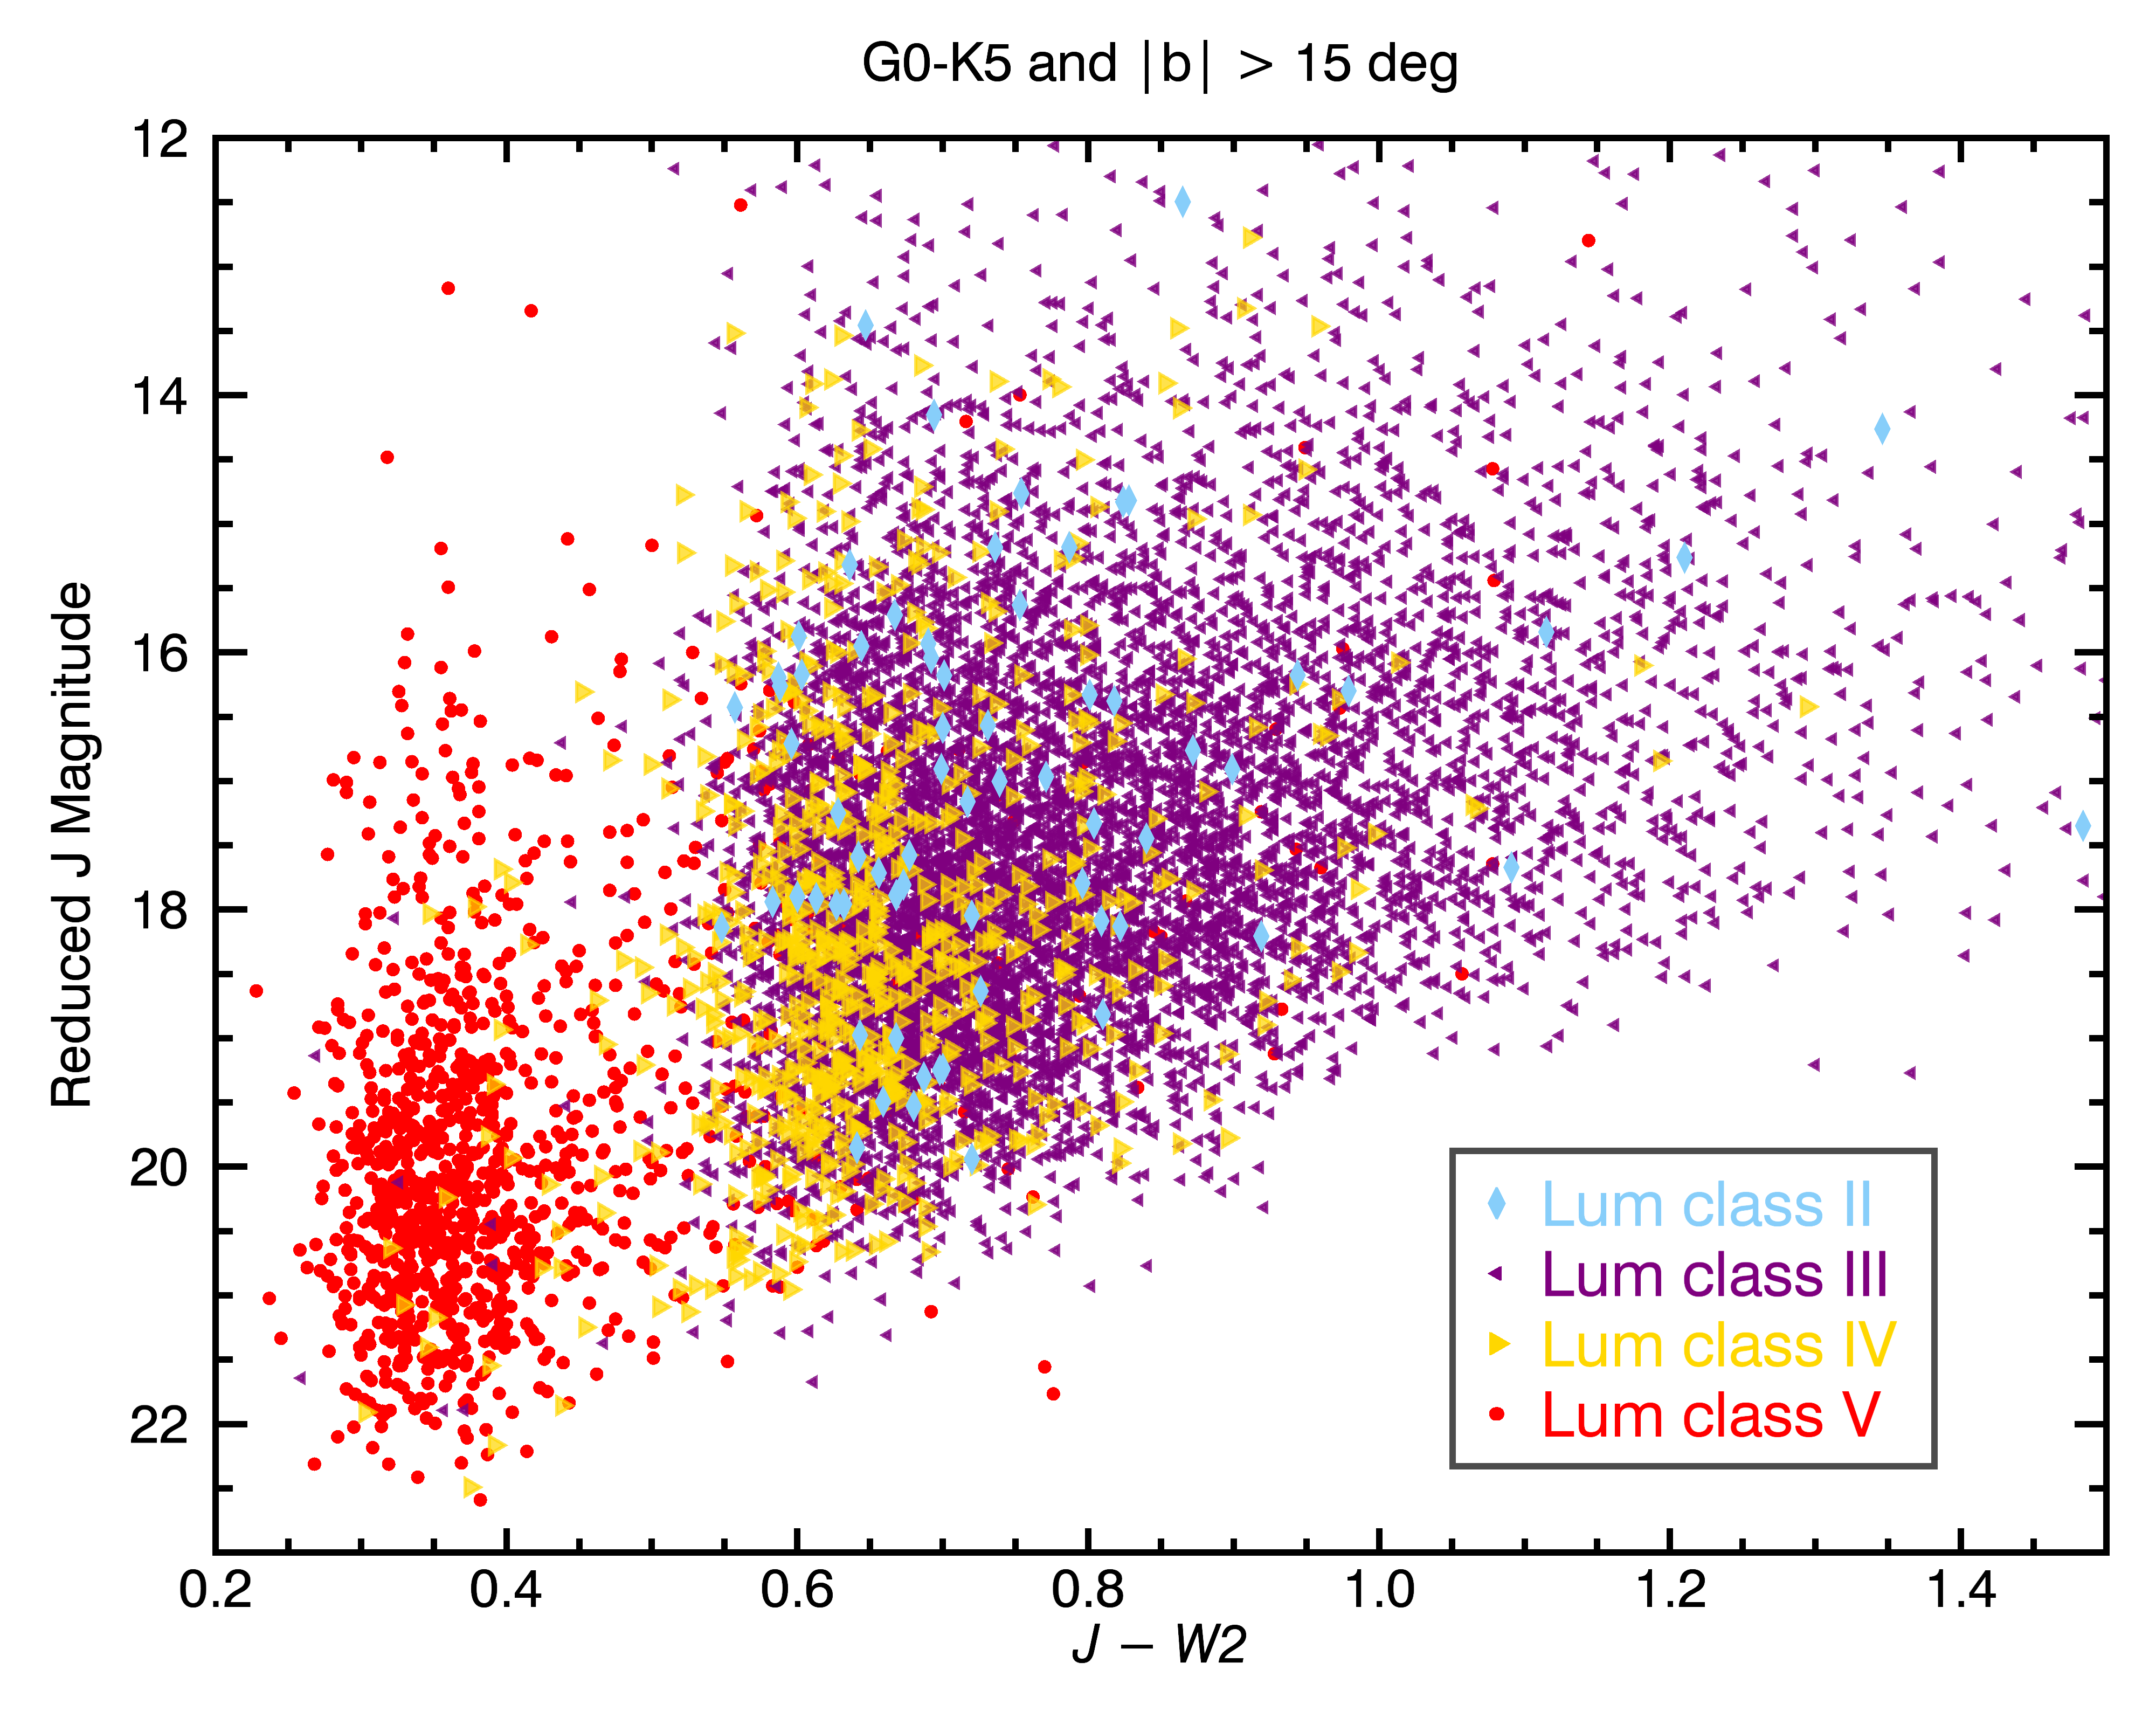
\includegraphics[width=1.0\textwidth,clip=true]{Figures/absolute_j/plot-J-W2-G0-K5-b15-rd-J.png}
\end{center}
\caption{The same as the previous figure, but for absolute $J$ band magnitudes using \textit{GAIA} DR1 parallaxes, validating the Michigan Spectral Atlas luminosity classes and the reduced proper motion approach.}\label{fig:reduced_j_jw2}
\end{figure*}